\documentclass[12pt, twoside]{article}
\usepackage[letterpaper, margin=1in, headsep=0.5in]{geometry}
\usepackage[english]{babel}
\usepackage[utf8]{inputenc}
\usepackage{amsmath}
\usepackage{amsfonts}
\usepackage{amssymb}
\usepackage{tikz}
\usetikzlibrary{quotes, angles}
\usepackage{graphicx}
\usepackage{enumitem}
\usepackage{multicol}

\newif\ifmeta
\metatrue %print standards and topics tags

\title{Regents Geometry}
\author{Chris Huson}
\date{February 2022}

\usepackage{fancyhdr}
\pagestyle{fancy}
\fancyhf{}
\renewcommand{\headrulewidth}{0pt} % disable the underline of the header
\raggedbottom

\fancyhead[LE]{\thepage}
\fancyhead[RO]{\thepage \\ Name: \hspace{4cm} \,\\}
\fancyhead[LO]{BECA / Dr. Huson / Geometry 7 Similarity}

\begin{document}

\subsubsection*{7.12 Similarity transformations \hfill CCSS.HSG.SRT.B.5}
\begin{enumerate}
\item Do Now: As shown, the chords $\overline{AE}$ and $\overline{BD}$ intersect at $C$, given $\triangle ABC \sim \triangle DEC$.
\begin{multicols}{2}
  \begin{enumerate}
    \item Given $BC=3$, and $EC=6$. Find the scale factor $k$.
    \item $AC=4$, find $CD$.
    \item Which angle is congruent to $\angle E$? \vspace{1cm}
  \end{enumerate}
  \begin{flushright}
    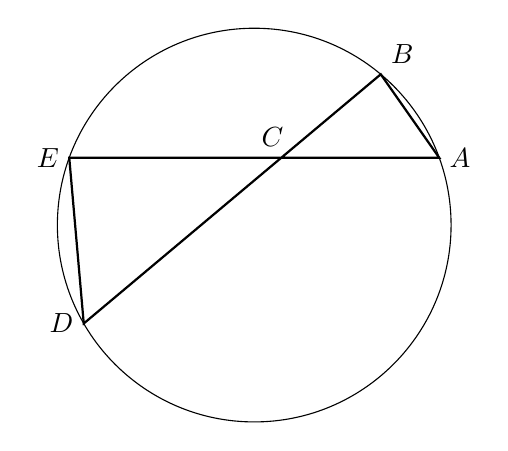
\begin{tikzpicture}[scale=.5]
      \draw (0,0) circle[radius=5];
      \draw [thick]
      (20:5) node[right] {$A$}--
      (160:5) node[left] {$E$}--
      (210:5) node[left] {$D$}--
      (50:5) node[above right] {$B$}--cycle;
      \draw (75:1.8) node[above] {$C$};
    \end{tikzpicture}
  \end{flushright}
\end{multicols}

\subsubsection*{Definition: Symmetry}
``Symmetry is a type of invariance: the property that a mathematical object remains unchanged under a set of operations or transformations.
\dots a symmetry is a mapping of [an] object onto itself." (Wikipedia, Symmetry in mathematics) \vspace{0.5cm}



\end{enumerate}
\end{document}
